% Figure 1: the architecture of bayesEfron 0.4.0, from the estimates to the
% reported quantities. Compile on its own:  pdflatex fig1_architecture
% (the standalone class writes fig1_architecture.pdf, which main.tex includes
% at the text width of the preprint, 137 mm, so the figure is drawn at about
% that width).
\documentclass[tikz,border=1.5pt]{standalone}
\usepackage[T1]{fontenc}
\usepackage{helvet}
\renewcommand{\familydefault}{\sfdefault}
\usepackage{amsmath}
\usetikzlibrary{positioning,arrows.meta,calc}
\definecolor{inkA}{HTML}{1A1A1A}
\definecolor{inkB}{HTML}{4D4D4D}
\definecolor{inkC}{HTML}{767676}
\definecolor{okblue}{HTML}{0072B2}
\definecolor{okverm}{HTML}{D55E00}
\definecolor{okgreen}{HTML}{009E73}
\definecolor{fillblue}{HTML}{EFF5FA}
\definecolor{fillgrey}{HTML}{F4F4F2}
\definecolor{fillverm}{HTML}{FBF4EF}
\definecolor{fillgreen}{HTML}{EEF7F3}
\newcommand{\head}[1]{{\fontsize{7.8}{9.2}\selectfont\bfseries #1}}
\newcommand{\note}[1]{{\fontsize{6.8}{8.1}\selectfont\color{inkB} #1}}
\newcommand{\code}[1]{{\fontsize{7.0}{8.3}\selectfont\ttfamily #1}}
\begin{document}
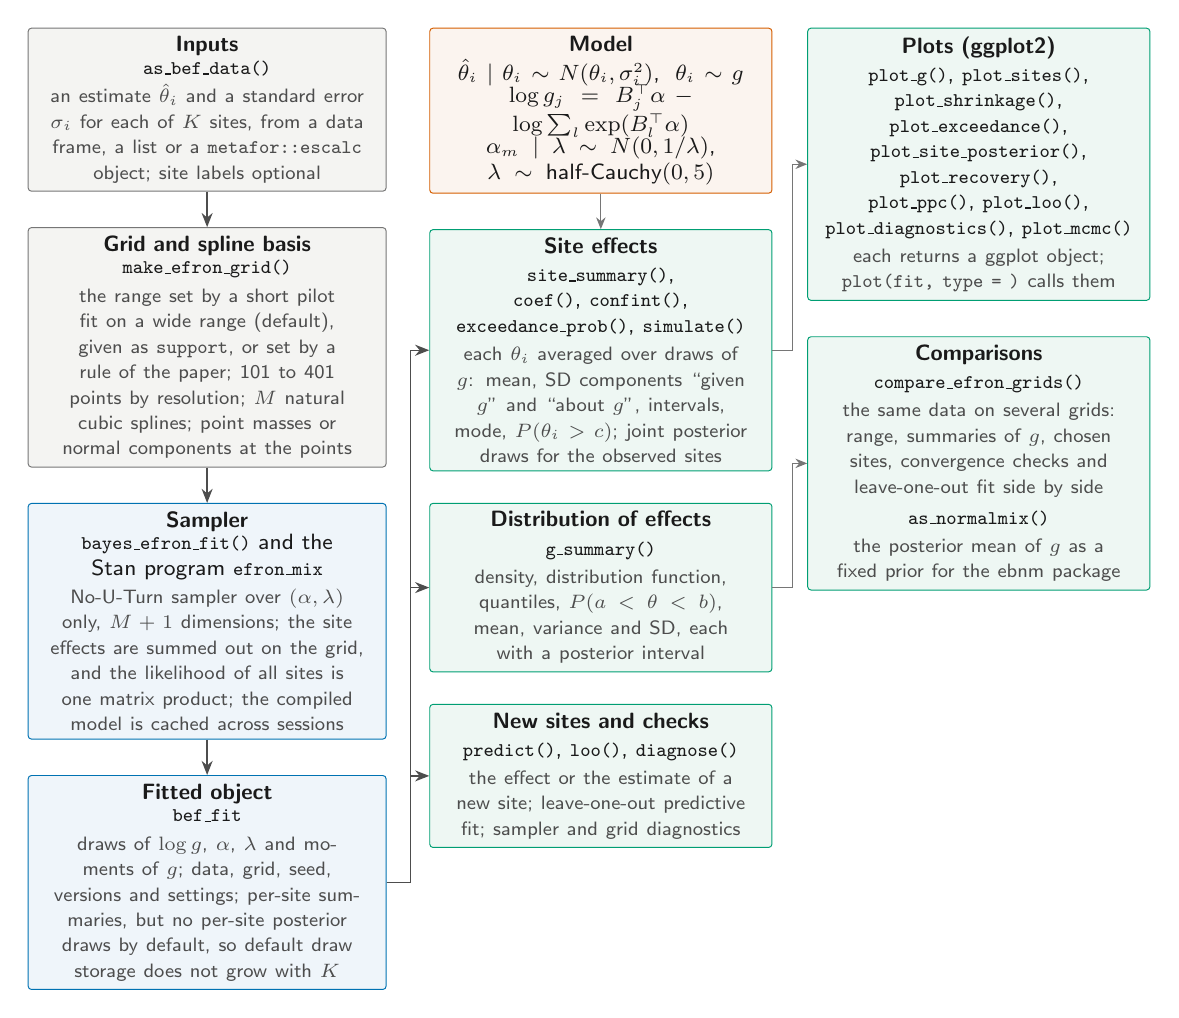
\begin{tikzpicture}[x=1mm, y=1mm,
  font=\fontsize{7.8}{9.2}\selectfont,
  every node/.style={text=inkA},
  box/.style={draw=inkC, line width=0.35pt, rounded corners=1.2pt, align=center,
              inner xsep=3.5pt, inner ysep=3pt, fill=white, anchor=north},
  stage/.style={box, fill=fillgrey, text width=43mm},
  core/.style={box, fill=fillblue, draw=okblue, text width=43mm},
  prod/.style={box, fill=fillgreen, draw=okgreen, text width=41mm},
  side/.style={box, fill=fillverm, draw=okverm, text width=41mm},
  arr/.style={-{Stealth[length=1.8mm,width=1.4mm]}, line width=0.5pt, draw=inkB},
  thin/.style={-{Stealth[length=1.5mm,width=1.2mm]}, line width=0.4pt, draw=inkC}
]
% ---------------- column 1: from the data to the fitted object ----------------
\node[stage] (input) at (0,0) {%
  \head{Inputs}\\[-1pt] \code{as\_bef\_data()}\\[1pt]
  \note{an estimate $\hat\theta_i$ and a standard error $\sigma_i$ for each of $K$ sites, from a data frame, a list or a \code{metafor::escalc} object; site labels optional}};
\node[stage] (grid) at ($(input.south)+(0,-4.5)$) {%
  \head{Grid and spline basis}\\[-1pt] \code{make\_efron\_grid()}\\[1pt]
  \note{the range set by a short pilot fit on a wide range (default), given as \code{support}, or set by a rule of the paper; 101 to 401 points by resolution; $M$ natural cubic splines; point masses or normal components at the points}};
\node[core] (stan) at ($(grid.south)+(0,-4.5)$) {%
  \head{Sampler}\\[-1pt] \code{bayes\_efron\_fit()} and the Stan program \code{efron\_mix}\\[1pt]
  \note{No-U-Turn sampler over $(\alpha,\lambda)$ only, $M+1$ dimensions; the site effects are summed out on the grid, and the likelihood of all sites is one matrix product; the compiled model is cached across sessions}};
\node[core] (fit) at ($(stan.south)+(0,-4.5)$) {%
  \head{Fitted object}\\[-1pt] \code{bef\_fit}\\[1pt]
  \note{draws of $\log g$, $\alpha$, $\lambda$ and moments of $g$; data, grid, seed, versions and settings; per-site summaries, but no per-site posterior draws by default, so default draw storage does not grow with $K$}};
% ---------------- column 2: the model and what is computed from the draws ----
\node[side] (model) at (50,0) {%
  \head{Model}\\[1pt]
  $\hat\theta_i\mid\theta_i\sim N(\theta_i,\sigma_i^2)$, \ $\theta_i\sim g$\\[-1pt]
  $\log g_j = B_j^{\top}\alpha - \log\textstyle\sum_l \exp(B_l^{\top}\alpha)$\\[-1pt]
  $\alpha_m\mid\lambda\sim N(0,1/\lambda)$, \ $\lambda\sim\text{half-Cauchy}(0,5)$};
\node[prod] (sites) at ($(model.south)+(0,-4.5)$) {%
  \head{Site effects}\\[1pt]
  \code{site\_summary()}, \code{coef()}, \code{confint()}, \code{exceedance\_prob()}, \code{simulate()}\\[1pt]
  \note{each $\theta_i$ averaged over draws of $g$: mean, SD components ``given $g$'' and ``about $g$'', intervals, mode, $P(\theta_i > c)$; joint posterior draws for the observed sites}};
\node[prod] (gsum) at ($(sites.south)+(0,-4)$) {%
  \head{Distribution of effects}\\[1pt]
  \code{g\_summary()}\\[1pt]
  \note{density, distribution function, quantiles, $P(a<\theta<b)$, mean, variance and SD, each with a posterior interval}};
\node[prod] (pred) at ($(gsum.south)+(0,-4)$) {%
  \head{New sites and checks}\\[1pt]
  \code{predict()}, \code{loo()}, \code{diagnose()}\\[1pt]
  \note{the effect or the estimate of a new site; leave-one-out predictive fit; sampler and grid diagnostics}};
% ---------------- column 3: plots and comparisons ----------------
\node[prod] (plots) at (98,0) {%
  \head{Plots (ggplot2)}\\[1pt]
  \code{plot\_g()}, \code{plot\_sites()}, \code{plot\_shrinkage()}, \code{plot\_exceedance()}, \code{plot\_site\_posterior()}, \code{plot\_recovery()}, \code{plot\_ppc()}, \code{plot\_loo()}, \code{plot\_diagnostics()}, \code{plot\_mcmc()}\\[1pt]
  \note{each returns a ggplot object; \code{plot(fit, type = )} calls them}};
\node[prod] (cmp) at ($(plots.south)+(0,-4.5)$) {%
  \head{Comparisons}\\[1pt]
  \code{compare\_efron\_grids()}\\[1pt]
  \note{the same data on several grids: range, summaries of $g$, chosen sites, convergence checks and leave-one-out fit side by side}\\[2pt]
  \code{as\_normalmix()}\\[1pt]
  \note{the posterior mean of $g$ as a fixed prior for the ebnm package}};
% ---------------- arrows ----------------
\draw[arr] (input) -- (grid);
\draw[arr] (grid) -- (stan);
\draw[arr] (stan) -- (fit);
\draw[arr] (fit.east) -- ++(3,0) |- (sites.west);
\draw[arr] (fit.east) -- ++(3,0) |- (gsum.west);
\draw[arr] (fit.east) -- ++(3,0) |- (pred.west);
\draw[thin] (model.south) -- (sites.north);
\draw[thin] (sites.east) -- ++(2.5,0) |- (plots.west);
\draw[thin] (gsum.east) -- ++(2.5,0) |- (cmp.west);
\end{tikzpicture}
\end{document}
